\documentclass{article}

\def\npart{III}
\def\nyear{2018}
\def\nterm{Michaelmas}
\def\nlecturer{Dr. S. Barbina}
\def\ncourse{Model Theory}
\def\draft{Ongoing course, rough}
\usepackage{mathrsfs}
\usepackage{imakeidx}
\usepackage{marginnote}
\ifx \nauthor\undefined
  \def\nauthor{Bhavik Mehta}
\else
\fi

\author{Based on lectures by \nlecturer \\\small Notes taken by \nauthor}
\date{\nterm\ \nyear}
\title{Part \npart\ -- \ncourse}

\usepackage[utf8]{inputenc}
\usepackage{amsmath}
\usepackage{amsthm}
\usepackage{amssymb}
\usepackage{enumerate}
\usepackage{mathtools}
\usepackage{graphicx}
\usepackage[dvipsnames]{xcolor}
\usepackage{tikz}
\usepackage{wrapfig}
\usepackage{centernot}
\usepackage{float}
\usepackage{braket}
\usepackage[hypcap=true]{caption}
\usepackage{enumitem}
\usepackage[colorlinks=true, linkcolor=mblue]{hyperref}
\usepackage[nameinlink,noabbrev]{cleveref}
\usepackage{nameref}
\usepackage[margin=1.5in]{geometry}

% Theorems
\theoremstyle{definition}
\newtheorem*{aim}{Aim}
\newtheorem*{axiom}{Axiom}
\newtheorem*{claim}{Claim}
\newtheorem*{cor}{Corollary}
\newtheorem*{conjecture}{Conjecture}
\newtheorem*{defi}{Definition}
\newtheorem*{eg}{Example}
\newtheorem*{ex}{Exercise}
\newtheorem*{fact}{Fact}
\newtheorem*{law}{Law}
\newtheorem*{lemma}{Lemma}
\newtheorem*{notation}{Notation}
\newtheorem*{prop}{Proposition}
\newtheorem*{question}{Question}
\newtheorem*{rrule}{Rule}
\newtheorem*{thm}{Theorem}
\newtheorem*{assumption}{Assumption}

\newtheorem*{remark}{Remark}
\newtheorem*{warning}{Warning}
\newtheorem*{exercise}{Exercise}

% \newcommand{\nthmautorefname}{Theorem}

\newtheorem{nthm}{Theorem}[section]
\newtheorem{nlemma}[nthm]{Lemma}
\newtheorem{nprop}[nthm]{Proposition}
\newtheorem{ncor}[nthm]{Corollary}
\newtheorem{ndef}[nthm]{Definition}

% Special sets
\newcommand{\C}{\mathbb{C}}
\newcommand{\N}{\mathbb{N}}
\newcommand{\Q}{\mathbb{Q}}
\newcommand{\R}{\mathbb{R}}
\newcommand{\Z}{\mathbb{Z}}

\newcommand{\abs}[1]{\left\lvert #1\right\rvert}
\newcommand{\norm}[1]{\left\lVert #1\right\rVert}
\renewcommand{\vec}[1]{\boldsymbol{\mathbf{#1}}}

\let\Im\relax
\let\Re\relax

\DeclareMathOperator{\Im}{Im}
\DeclareMathOperator{\Re}{Re}
\DeclareMathOperator{\id}{id}

\definecolor{mblue}{rgb}{0., 0.05, 0.6}

\makeindex[intoc]

% preamble

\reversemarginpar

\let\oldmodels\models
\let\models\vDash
\let\nModels\nvDash

\setcounter{section}{-1}

\DeclareMathOperator{\Mod}{Mod}
\DeclareMathOperator{\Th}{Th}
\DeclarePairedDelimiter\ceil{\lceil}{\rceil}
\DeclarePairedDelimiter\floor{\lfloor}{\rfloor}

\newtheorem{nremark}[nthm]{Remark}
\newtheorem{nexample}[nthm]{Example}
\newtheorem{nexercise}[nthm]{Exercise}
\newtheorem{nfact}[nthm]{Fact}
\newtheorem{nnotation}[nthm]{Notation}

%\newtheorem{manualtheoreminner}{Theorem}
%\newenvironment{manualtheorem}[1]{%
%    \renewcommand\themanualtheoreminner{#1}%
%    \manualtheoreminner
%}{\endmanualtheoreminner}

% and here we go!

\begin{document}
\maketitle

\tableofcontents

\clearpage
\section{Introduction}
\marginnote{\emph{Lecture 1}}[0cm]
Model theory is a part of logic that began by looking at algebraic objects such as groups and combinatorial objects such like graphs, described in formal language.
The basic question in model theory is: `how powerful is our description of these objects to pin them down'?
In Logic and Set Theory, the focus was on what was provable from a theory and language, but here we focus on whether or not a model exists.

\section{Languages and structures}
\begin{ndef}[Language]\label{def:1.1}\index{language}\hypertarget{def:lang}
  A \textbf{language} $L$ consists of
  \begin{enumerate}[label=(\roman*)]
    \item a set $\mathscr{F}$ of function symbols, and for each $f \in \mathscr{F}$ a positive integer $m_f$ the \textbf{arity} of $f$.
    \item a set $\mathscr{R}$ of relation symbols, and for each $R \in \mathscr{R}$, a positive integer $m_R$.
    \item a set $\mathscr{C}$ of constant symbols.
  \end{enumerate}
  Note: each of $\mathscr{F}, \mathscr{R}$ and $\mathscr{C}$ can be empty.
\end{ndef}
\begin{eg}
  \hypertarget{def:lgp}Take $L = \{\{\cdot , ^{-1}\}, \{1\}\}$, for $\cdot$ a binary function and $^{-1}$ an unary function, $1$ a constant. This is the \hyperlink{def:lang}{language} of groups, call it $L_{gp}$.
  Also, $L_{lo} = \{<\}$ a single binary relation, for linear orders.
\end{eg}

\begin{ndef}[$L$-structure]\label{def:1.2}\index{L-structure@$L$-structure}\hypertarget{def:lstr}
  Given a \hyperlink{def:lang}{language} $L$, say, an \textbf{$L$-structure} consists of
  \begin{enumerate}[label=(\roman*)]
    \item a set $M$, the \textbf{domain}
    \item for each $f \in \mathscr{F}$, a function $f^\mathcal{M} : M^{m_f} \to M$.
    \item for each $R \in \mathscr{R}$, a relation $R^\mathcal{M} \subseteq M^{m_R}$.
    \item for each $c \in \mathscr{C}$, an element $c^\mathcal{M} \in M$.
  \end{enumerate}
  $f^M, R^M, c^M$ are the \textbf{interpretations} of $f,R,c$ respectively.
\end{ndef}
\begin{nremark}\label{rem:1.3}
  We often fail to distinguish between the \hyperlink{def:lang}{symbols} in $L$ and their \hyperlink{def:lstr}{interpretations} in a \hyperlink{def:lstr}{structure}, if the interpretations are clear from the context.
\end{nremark}

We may write $\mathcal{M} = \langle M, \mathscr{F}, \mathscr{R}, \mathscr{C} \rangle$.

\begin{nexample}\label{eg:1.4}\leavevmode
  \begin{enumerate}[label=(\alph*)]
    \item $\mathcal{R} = \langle \mathbb{R}^+, \{\cdot, ^{-1}\}, 1 \rangle$ is an \hyperlink{def:lgp}{$L_{gp}$}-\hyperlink{def:lstr}{structure}.
    \item $\mathcal{Z} = \langle \mathbb{Z}, \{+, -\}, 0 \rangle$ is an $L_{gp}$-structure.
    \item $\mathcal{Q} = \langle \mathbb{Q}, < \rangle$ is an \hyperlink{def:lgp}{$L_{lo}$}-structure.
  \end{enumerate}
\end{nexample}
\begin{ndef}[Embedding]\label{def:1.5}\index{embedding}\hypertarget{def:embedding}
  Let $L$ be a \hyperlink{def:lang}{language}, let $\mathcal{M}, \mathcal{N}$ be \hyperlink{def:lstr}{$L$-structures}.
  An \textbf{embedding} of $\mathcal{M}$ into $\mathcal{N}$ is a one-to-one mapping $\alpha: M \to N$ such that
  \begin{enumerate}[label=(\roman*)]
    \item for all $f \in \mathscr{F}$, and $a_1, \dotsc, a_{m_f} \in M$,
      \begin{equation*}
        \alpha(f^\mathcal{M}(a_1, \dotsc, a_{n_f})) = f^\mathcal{N}(\alpha(a_1), \dotsc, \alpha(a_{n_f}))
      \end{equation*}
      \begin{center}
        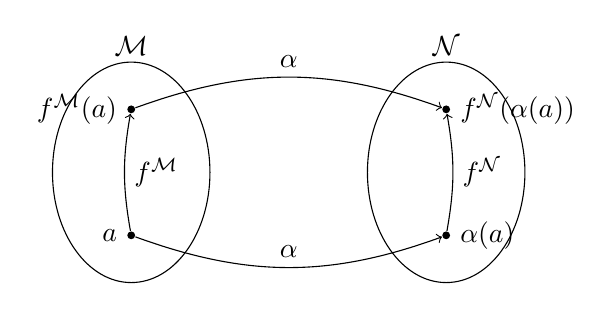
\begin{tikzpicture}[scale=1]
          \node at (-2, 1.6) {$\mathcal{M}$};
          \node at (2, 1.6) {$\mathcal{N}$};
          \draw (-2, 0) circle [x radius=10mm, y radius=14mm];
          \node [circle, inner sep=1pt, fill=black, label=left:$a$] (a) at (-2, -0.8) {};
          \node [circle, inner sep=1pt, fill=black, label=left:$f^\mathcal{M}(a)$] (fa) at (-2, 0.8) {};
          \draw (2, 0) circle [x radius=10mm, y radius=14mm];
          \node [circle, inner sep=1pt, fill=black, label=right:$\alpha(a)$] (aa) at (2, -0.8) {};
          \node [circle, inner sep=1pt, fill=black, label=right:$f^\mathcal{N}(\alpha(a))$] (faa) at (2, 0.8) {};
          \draw [->] (a) to [bend right=20] node[above]{$\alpha$} (aa);
          \draw [->] (fa) to [bend left=20] node[above]{$\alpha$} (faa);
          \draw [->] (a) to [bend left=10] node[right]{$f^\mathcal{M}$} (fa);
          \draw [->] (aa) to [bend right=10] node[right]{$f^\mathcal{N}$} (faa);
        \end{tikzpicture}
      \end{center}
    \item for all $R \in \mathscr{R}$, and $a_1, \dotsc, a_{n_R} \in M$
      \begin{equation*}
        (a_1, \dotsc, a_{n_R}) \in R^\mathcal{M} \iff (\alpha(a_1), \dotsc, \alpha(a_{n_R})) \in R^\mathcal{N}
      \end{equation*}
    \item for all $c \in \mathscr{C}$, $\alpha(c^\mathcal{M}) = c^\mathcal{N}$.
  \end{enumerate}
  An \textbf{isomorphism} of $\mathcal{M}$ into $\mathcal{N}$ is a surjective embedding (onto).
\end{ndef}

\begin{nexercise}\label{ex:1.6}
  Let $G_1, G_2$ be groups, regarded as \hyperlink{def:lgp}{$L_{gp}$}-structures.
  Check that $G_1 \simeq G_2$ in the usual algebra sense if and only if there is an \hyperlink{def:embedding}{isomorphism} $\alpha: G_1 \to G_2$ in the sense of \cref{def:1.5}.
\end{nexercise}

\clearpage
\section{Review: Terms, formulae and their interpretations}
In addition to the \hyperlink{def:lang}{symbols} of $L$, we also have
\begin{enumerate}[label=(\roman*)]
  \item infinitely many variables $\{x_i\}_{i \in I}$
  \item logical connectives $\wedge, \neg$ (also expresses $\vee, \implies, \iff$)
    \item quantifier $\exists$ (also expresses $\forall$)
    \item $(\phantom{-},\phantom{-})$
    \item equality symbol $=$
\end{enumerate}

\begin{ndef}[\hypertarget{def:lterm}{$L$-terms}]\label{def:2.1}
  \index{L-term@$L$-term}\textbf{$L$-terms} are defined recursively as follows:
  \begin{itemize}[label=--]
    \item any variable $x_i$ is a term
    \item any constant symbol is a term
    \item for any $f \in \mathscr{F}$, $f(t_1, \dotsc, t_{m_f})$ for any terms $t_1, \dotsc, t_{m_f}$ is a term
    \item nothing else is a term
  \end{itemize}
\end{ndef}

Notation: we write $t(x_1, \dotsc, x_m)$ to mean that the variables appearing in $t$ are among $x_1, \dotsc, x_m$.
\begin{eg}
  \marginnote{\emph{Lecture 2}}[0cm]
  Take $\mathcal{R} = \langle \mathbb{R}^*, \{\cdot, ^{-1}\}, 1 \rangle$.
  Then $\cdot ( \cdot(x_1, x_2), x_3)$ is a \hyperlink{def:lterm}{term}, usually written $(x_1 \cdot x_2) \cdot x_3$.
  Also, $(\cdot (1, x_1))^{-1}$ is a \hyperlink{def:lterm}{term}, written $(1\cdot x)^{-1}$
\end{eg}
\begin{ndef}\label{def:2.2}
  If $\mathcal{M}$ is an \hyperlink{def:lstr}{$L$-structure}, to each \hyperlink{def:lterm}{$L$-term} $t(x_1, \dotsc, x_k)$ we assign a function
  a function $t^\mathcal{M}: M^k \to M$ defined as follows:
  \begin{enumerate}[label=(\roman*)]
    \item If $t = x_i$, $t^\mathcal{M}[a_1, \dotsc, a_k] = a_i$
    \item If $t = c$, $t^\mathcal{M}[a_1, \dotsc, a_k] = c^\mathcal{M}$.
    \item If $t = f(t(x_1, \dotsc, x_k), \dotsc, t_{m_f}(x_1, \dotsc, x_k))$,
      \begin{equation*}
        t^\mathcal{M}(a_1, \dotsc, a_k) = f^\mathcal{M}(t_1^\mathcal{M}(a_1, \dotsc, a_k), \dotsc, t^\mathcal{M}_{m_f}(a_1, \dotsc, a_k))
      \end{equation*}
  \end{enumerate}
\end{ndef}

Notice in $L_{gp}$, the term $x_2 \cdot x_3$ can be described as $t_1(x_1, x_2, x_3)$ or $t_2(x_1, x_2, x_3, x_4)$, or infinitely many other ways.
Then $t_1$ is assigned to $t_1^\mathcal{M}: M^3 \to M$, with $(a_1, a_2, a_3) \mapsto (a_2, a_3)$, and $t_2$ is assigned to $t_2^\mathcal{M} : M^4 \to M$, with $(a_1, a_2, a_3, a_4) \mapsto a_2 \cdot a_3$.
\begin{nfact}\label{fact:2.3}
  Let $\mathcal{M}, \mathcal{N}$ be \hyperlink{def:lstr}{$L$-structures}, and let $\alpha: \mathcal{M} \to \mathcal{N}$ be an \hyperlink{def:embedding}{embedding}.
  For any \hyperlink{def:lterm}{$L$-term} $t(x_1, \dotsc, x_k)$ and $a_1, \dotsc, a_k \in M$ we have
  \begin{equation*}
    \alpha(t^\mathcal{M}(a_1, \dotsc, a_k)) = t^\mathcal{N}(\alpha(a_1), \dotsc, \alpha(a_k))
  \end{equation*}
\end{nfact}
\begin{proof}
  By induction on the complexity of $t$. Let $\bar{a} = (a_1, \dotsc, a_k)$ and $\bar{x} = (x_1, \dotsc, x_k)$.
  Then
  \begin{enumerate}[label=(\roman*)]
    \item if $t = x_i$, then $t^\mathcal{M}(\bar{a}) = a_i$, and $t^\mathcal{N}(\alpha(a_1), \dotsc, \alpha(a_k)) = \alpha(a_i)$, so the conclusion holds.
    \item if $t = c$ a constant, then $t^\mathcal{M}(\bar{a}) = c^\mathcal{M}$, and $t^\mathcal{N}(\alpha(\bar{a})) = c^\mathcal{N}$, and $\alpha(c^\mathcal{M}) = c^\mathcal{N}$, as required.
    \item if $t = f(t_1(\bar{x}),\dotsc, t_{m_f}(\bar{x}))$, then
      \begin{equation*}
        \alpha(f^\mathcal{M}(t_1^\mathcal{M}(\bar{a}), \dotsc, t_{m_f}^\mathcal{M}(\bar{a}))) = f^\mathcal{N}(\alpha(t_1^\mathcal{M}(\bar{a})), \dotsc, \alpha(t_{m_f}^\mathcal{M}(\bar{a})))
      \end{equation*}
      since $\alpha$ is an embedding.
      $t_1(\bar{x}), \dotsc, t_{m_f}(\bar{x})$ have lower complexity than $t$, so inductive hypothesis applies.
  \end{enumerate}
\end{proof}
\begin{nexample}\label{eg:2.4}
  Exercise: conclude the proof of \cref{fact:2.3}.
\end{nexample}
\begin{ndef}[Atomic formula]\label{def:2.5}\index{formula!atomic}\hypertarget{def:atomform}
  The set of \textbf{atomic formulas} of $L$ is defined as follows
  \begin{enumerate}[label=(\roman*)]
    \item if $t_1, t_2$ are $L$-terms, then $t_1 = t_2$ is an atomic formula
    \item if $R$ is a relation symbol and $t_1, \dotsc, t_{m_R}$ are terms, then $R(t_1, \dotsc, t_{m_R})$ is an atomic formula
    \item nothing else is an atomic formula.
  \end{enumerate}
\end{ndef}
\begin{ndef}[Formula]\label{def:2.6}\index{formula}\hypertarget{def:form}
  The set of \textbf{$L$-formulas} is defined as follows
  \begin{enumerate}[label=(\roman*)]
    \item any \hyperlink{def:atomform}{atomic formula} is an $L$-formula
    \item if $\phi$ is an $L$-formula, then so is $\neg \phi$
    \item if $\phi$ and $\psi$ are $L$-formulas, then so is $\phi \wedge \psi$
    \item if $\phi$ is an $L$-formula, for any $i \geq 1$, $\exists x_i \phi$ is an $L$-formula
    \item nothing else is an $L$-formula
  \end{enumerate}
\end{ndef}
\begin{eg}
  In $L_{gp}$, $x_1 \cdot x_1 = x_2$ and $x_1 \cdot x_2 = 1$ are \hyperlink{def:form}{atomic formulas}, and $\exists x_1 (x_1 \cdot x_2) = 1$ is an $L_{gp}$-formula.
\end{eg}
\index{free variable}\index{bound variable}\hypertarget{def:free}A variable occurs freely in a formula if it does not occur within the scope of a quantifier $\exists$ (the variable is \textbf{free}). Otherwise the variable is \textbf{bound}. For instance, in $\exists x_1 (x_1 \cdot x_2) = 1$, $x_1$ is bound and $x_2$ is free.

\textbf{Important convention:} no variable occurs both \hyperlink{def:free}{freely} and as a bound variable in the same formula.

\index{sentence}\hypertarget{def:sentence}A \textbf{sentence} is a \hyperlink{def:form}{formula} with no \hyperlink{def:free}{free} variables. $\exists x_1 \exists x_2 (x_1 \cdot x_2 = 1)$ is an $L_{gp}$-sentence.

Notation: $\phi(x_1, \dotsc, x_k)$ means that the free variables in $\phi$ are among $x_1, \dotsc, x_k$.

\begin{ndef}[$\models$]\label{def:2.7}\index{$\models$}\hypertarget{def:models}
  Let $\phi(x_1, \dotsc, x_k)$ be an $L$-formula, let $\mathcal{M}$ be an $L$-structure, and let $\bar{a} = (a_1, \dotsc, a_k)$ be elements of $\mathcal{M}$.
  We define $\mathcal{M} \models \phi(\bar{a})$ as follows.
  \begin{enumerate}[label=(\roman*)]
    \item if $\phi$ is $t_1 = t_2$, then $\mathcal{M} \models \phi(\bar{a})$ if and only if $t_1^\mathcal{M}(\bar{a}) = t_2^\mathcal{M}(\bar{a})$.
    \item if $\phi$ is $R(t_1, \dotsc, t_{m_k})$ then $\mathcal{M} \models \phi(\bar{a})$ iff
      \begin{equation*}
        (t_1^\mathcal{M}(\bar{a}),\dotsc,t_{m_k}^\mathcal{M}(\bar{a})) \in R^\mathcal{M}.
      \end{equation*}
    \item if $\phi$ is $\psi \wedge \chi$, then $\mathcal{M} \models \phi(\bar{a})$ iff $\mathcal{M} \models \psi(\bar{a})$ and $\mathcal{M} \models \chi(\bar{a})$.
    \item if $\phi = \neg \psi$ then $\mathcal{M} \models \phi(\bar{a})$ iff $\mathcal{M} \nModels \psi(\bar{a})$. (this is well-defined since $\psi(\bar{a})$ is shorter than $\phi(\bar{a})$)
    \item if $\phi$ is $\exists x_j: \chi(x_1, \dotsc, x_k, x_j)$ (where $x_j \neq x_i$ for $i = 1, \dotsc, k$).
      Then $\mathcal{M} \models \phi(\bar{a})$ iff there is $b \in \mathcal{M}$ such that $\mathcal{M} \models \chi(a_1, \dotsc, a_k, b)$.
  \end{enumerate}
\end{ndef}
\begin{eg}
  For $\mathcal{R} = \langle \mathbb{R}^*,\cdot, ^{-1}, 1\rangle$, $\phi(x_1) = \exists x_2 (x_2 \cdot x_2) = x_1$ then $\mathcal{R} \hyperlink{def:models}{\models} \phi(1)$ but $\mathcal{R} \nModels \phi(-1)$.
\end{eg}
\begin{nnotation}[Useful abbreviations]\label{not:2.8}
  We write
  \begin{itemize}[label=--]
    \item $\phi \vee \psi$ for $\neg(\neg\phi \wedge \neg\psi)$
    \item $\phi \to \psi$ for $\neg \phi \vee \psi$
    \item $\phi \leftrightarrow \psi$ for $(\phi \to \psi) \wedge (\psi \to \phi)$
    \item $\forall x_i\ \phi$ for $\neg \exists x_i\ (\neg \phi)$
  \end{itemize}
\end{nnotation}
\begin{nprop}\label{prop:2.9}
  Let $\mathcal{M}, \mathcal{N}$ be \hyperlink{def:lstr}{$L$-structures}, let $\alpha: \mathcal{M} \to \mathcal{N}$ be an \hyperlink{def:embedding}{embedding}.
  Let $\phi(\bar{x})$ be \hyperlink{def:atomform}{atomic} and $\bar{a} \in M^{|\bar{x}|}$, then
  \begin{equation*}
    M \hyperlink{def:models}{\models} \phi(\bar{a}) \iff \mathcal{N} \models \phi(\alpha(\bar{a})).
  \end{equation*}
\end{nprop}

Question: If $\phi$ is an \hyperlink{def:form}{$L$-formula}, not necessarily atomic, does \cref{prop:2.9} hold?

\marginnote{\emph{Lecture 3}}[0cm]
\begin{proof}[Proof of \cref{prop:2.9}]
  Cases:
  \begin{enumerate}[label=(\roman*)]
    \item $\phi(\bar{x})$ is of the form $t_1(\bar{x}) = t_2(\bar{x})$ where $t_1,t_2$ are terms.
      (Exercise: complete this case, using \cref{fact:2.3})
    \item $\phi(\bar{x})$ is of the form $R(t_1(\bar{x}), \dotsc, t_{m_R}(\bar{x}))$.
      Then $\mathcal{M} \hyperlink{def:models}{\models} R(t_1(\bar{a}), \dotsc, t_{m_R})$ if and only if...
      (Exercise: complete this case)
  \end{enumerate}
\end{proof}
\begin{nexercise}\label{ex:2.10}
  Show that \cref{prop:2.9} holds if $\phi(\bar{x})$ is a formula without quantifiers (a quantifier-free formula).
\end{nexercise}
\begin{nexample}\label{ex:2.11}
  Do \hyperlink{def:embedding}{embeddings} preserve \emph{all} \hyperlink{def:form}{formulas}? No.
  Take $\mathcal{Z} = (\mathbb{Z}, <)$ and $\mathcal{Q} = (\mathbb{Q}, <)$ an \hyperlink{def:lgp}{$L_{lo}$}-\hyperlink{def:lstr}{structure}
  Then $\alpha: \mathbb{Z} \to \mathbb{Q}$ (inclusion) is an embedding, but
  \begin{gather}
    \phi(x_1, x_2) = \exists x_3\,(x_1 < x_3 \wedge x_3 < x_2). \\
    \mathcal{Q} \hyperlink{def:models}{\models} \phi(1,2) \text{ but } \mathcal{Z} \nModels \phi(1,2).
  \end{gather}
\end{nexample}
\begin{nfact}\label{fact:2.12}
  Let $\alpha: \mathcal{M} \to \mathcal{N}$ be an \hyperlink{def:embedding}{isomorphism}.
  Then if $\phi(\bar{x})$ is an \hyperlink{def:form}{$L$-formula} and $\bar{a} \in M^{|\bar{x}|}$, then
  \begin{equation*}
    \mathcal{M} \hyperlink{def:models}{\models} \phi(\bar{a}) \iff \mathcal{M} \models \phi(\alpha(\bar{a})).
  \end{equation*}
\end{nfact}
\begin{proof}
  Exercise.
\end{proof}

\clearpage
\section{Theories and elementarity}
Throughout, $L$ is a \hyperlink{def:lang}{language}, $\mathcal{M}, \mathcal{N}$ are \hyperlink{def:lstr}{$L$-structures}.
\begin{ndef}[$L$-theory]\label{def:3.1}\index{L-theory@$L$-theory}\hypertarget{def:ltheory}
  An \textbf{$L$-theory} $T$ is a set of \hyperlink{def:sentence}{$L$-sentences}.
  $\mathcal{M}$ is a \textbf{model} of $T$ if $\mathcal{M} \hyperlink{def:models}{\models} \sigma$ for all $\sigma \in T$. We write $\mathcal{M} \models T$.
  The class of all the models of $T$ is written $\Mod(T)$.
  The theory of $\mathcal{M}$ is the set
  \begin{equation*}
    \Th(\mathcal{M}) = \set{\sigma | \sigma \text{ is an } L\text{-\hyperlink{def:lstr}{structure} and } \mathcal{M} \models \sigma}.
  \end{equation*}
\end{ndef}
\begin{nexample}\label{eg:3.2}
  Let $T_{gp}$ be the set of \hyperlink{def:lgp}{$L_{gp}$}-\hyperlink{def:sentence}{sentences}.
  \begin{enumerate}[label=(\roman*)]
    \item $\forall x_1 x_2 x_3\, (x_1 \cdot (x_2 \cdot x_3) = (x_1 \cdot x_2) \cdot x_3)$
    \item $\forall x_1\, (x_1 \cdot 1 = 1 \cdot x_1 = x_1)$
    \item $\forall x_1\,(x_1 \cdot x_1^{-1} = x_1^{-1} \cdot x_1 = 1)$
  \end{enumerate}
\end{nexample}
Clearly for a group $G$, $G \hyperlink{def:models}{\models} T_{gp}$. For a specific $G$, clearly $\hyperlink{def:ltheory}{\Th(G)}$ is larger than $T_{gp}$!

\begin{ndef}\hypertarget{def:eleq}\index{elementarily equivalent}\label{def:3.3}
  $\mathcal{M}$ and $\mathcal{N}$ are \textbf{elementarily equivalent} if $\Th(\mathcal{M}) = \Th(\mathcal{N})$.
  We write $\mathcal{M} \equiv \mathcal{N}$.
  Clearly if $\mathcal{M} \simeq \mathcal{N}$, then $\mathcal{M} \equiv \mathcal{N}$ but if $\mathcal{M}$ and $\mathcal{N}$ are not isomorphic, establishing whether $\mathcal{M} \equiv \mathcal{N}$ can be highly non-trivial!

  We'll see $(\mathbb{Q}, <) \equiv (\mathbb{R}, <)$ as $L_{lo}$-structures.
\end{ndef}
\begin{ndef}\label{def:3.4}\leavevmode
  \begin{enumerate}[label=(\roman*)]
    \item an embedding $\beta: \mathcal{M} \to \mathcal{N}$ is \textbf{elementary} if for all formulas $\phi(\bar{x})$ and $\bar{a} \in M^{|\bar{x}|}$,
      \begin{equation*}
        \mathcal{M} \models \phi(\bar{a}) \iff \mathcal{N} \models \phi(\beta(\bar{a}))
      \end{equation*}
    \item if $M \subseteq N$ and $\operatorname{id}: \mathcal{M} \to \mathcal{N}$ is an embedding, then $\mathcal{M}$ is said to be a \textbf{substructure} of $\mathcal{N}$.
    \item if $M \subseteq N$ and $\operatorname{id}: \mathcal{M} \to \mathcal{N}$ is an elementary embedding, then $\mathcal{M}$ is said to be an \textbf{elementary substructure} of $\mathcal{N}$, written $\mathcal{M} \preccurlyeq \mathcal{N}$.
  \end{enumerate}
\end{ndef}
\begin{nexample}\label{eg:3.5}
  Consider $\mathcal{M} = [0,1] \subseteq \mathbb{R}$, an $L_{lo}$-structure, where $<$ is the usual order, and $\mathcal{N} = [0,2] \subseteq \mathbb{R}$ in the same way.
  Then $\mathcal{M} \simeq \mathcal{N}$ as $L_{lo}$-structures.
  Is $\mathcal{M} \equiv \mathcal{N}$? Yes they are isomorphic!

  Is $\mathcal{M} \subseteq \mathcal{N}$? Yes (the ordering $<$ coincides on $\mathcal{M}$ and $\mathcal{N}$.)
  But $\mathcal{M} \not\preccurlyeq \mathcal{N}$, since if $\phi(x) = \exists y (x < y)$, then
  \begin{equation*}
    \mathcal{N} \models \phi(1)\quad\text{and}\quad\mathcal{M} \nModels \phi(1).
  \end{equation*}
\end{nexample}
\begin{ndef}\label{def:3.6}
  Let $\mathcal{M}$ an $L$-structure, $A \subseteq M$, then
  \begin{equation*}
    L(A) \coloneqq L \cup \set{c_a : a \in A}
  \end{equation*}
  for $c_a$ each constant symbols.
  An interpretation of $\mathcal{M}$ as an $L$-structure extends to an interpretation of $\mathcal{M}$ as an $L(A)$-structure in the obvious way ($c_a^\mathcal{M} = a$).
  The elements of $A$ are called \textbf{parameters}.
  If $\mathcal{M}, \mathcal{N}$ are $L$-structures and $A \subseteq M \cap N$, then $\mathcal{M} \equiv_A \mathcal{N}$ when $\mathcal{M}, \mathcal{N}$ satisfy exactly the same $L(A)$ sentences.
\end{ndef}
\printindex
\end{document}
